\documentclass[10pt,handout,usepdftitle=false,envcountsect]{beamer}

\usepackage[utf8]{inputenc}
\usepackage[francais]{babel}
\usepackage[T1]{fontenc}
\usepackage{tikz}
\usepackage{tikzscale}
\usepackage{tikz-uml}
\usepackage{scalefnt}
\usepackage{calc}
\usepackage{verbatim}
\usepackage{pgf-pie}
\usetheme{Hannover}


% Title Page
\title{Gestion de performances de coureurs}
\author{Quentin Le Guennec}
\institute{Lycée Pierre Méchain Laon}
\date{\today}

\begin{document}
\section{Présentation}

\begin{frame}
    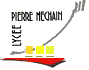
\includegraphics[scale=0.7]{pierre-mechain.png}
    \maketitle
\end{frame}

\subsection{Sommaire}
\frametitle{Sommaire}
\begin{frame}
    \tableofcontents
\end{frame}

\subsection{Introduction}
\begin{frame}
\frametitle{Naming utilisé}
\begin{description}
    \item[dbDial] Classe qui gère les dialogues avec la base de données
        \newline
    \item[CodeReader] Lecteur de code barre pour idenfier un adhérent grâce à sa carte.
        \newline
    \item[RFIDReader] Lecteur de badges par RFID pour attribuer à un coureur un ID
        \newline
    \item[Portique] Lecteur de badges par RFID qui permet de notifier le passage d'un coureur
        \newline
    \item[Michel] Désigne un participant, Adhérent ou non
\end{description}
\end{frame}


\subsection{Travail effectué}
\begin{frame}

\frametitle{Participants au projet}
    \begin{description}
        \item[Quentin Le Guennec] site web et de la base de données, aide générale
            \item[Classes]{CodeReader}
            \newline
        \item[Bastien Kopka] design du site web, analyse des documentations
            \item[Classes]{Portique, RFIDReader}
            \newline
        \item[Léo David] analyse des documentations
            \item[Classes]{Portique, RFIDReader}
            \newline
    \end{description}
\end{frame}

\begin{frame}
\frametitle{Répartition du temps}
    \begin{tikzpicture}[scale=0.5]
            \pie{12/Analyse des documentations, 15/Développement, 16/Analyse UML, 30/BDD et Serveur web, 27/Analyse du matériel}
    \end{tikzpicture}
\emph{Au total:} Environ 70 heures
\end{frame}

\subsection{Objectif du système}
\begin{frame}
\frametitle{Objectif du système}
\begin{itemize}
    \item Gérer le déroulement d'une course automatiquement
    \item Enregistrer les performances des coureurs
    \item Présenter sur un support de son choix les performances d'un coureur
\end{itemize}
\end{frame}
\section{Analyse UML}

% Config de tikz
\tikzumlset{font=\tiny}

\subsection{Use cases}
\begin{frame}
\frametitle{Diagramme de cas d'utilisation}
\begin{tikzpicture}
% Acteurs extérieurs
\umlactor[x=-2,y=4,below=0.3cm]{Adhérent}
\umlactor[x=-2,below=0.3cm]{Consultant}
\umlactor[x=-2,y=2,below=0.3cm]{Participant}
\umlinherit{Consultant}{Participant}
\umlinherit{Participant}{Adhérent}
\begin{umlsystem}[x=1.5]{Gestion de performances de coureurs}

% Acteurs intérieurs
\umlactor[x=5.7,y=1.5,below=0.3cm]{Base de données}

% Cas d'utilisations
\umlusecase[name=case1]{consulter performances}
\umlusecase[y=2,name=case3]{participer à une course}
\umlusecase[x=4,y=3.5,name=case4]{enregistrer coureur}
\umlusecase[y=4,name=case5]{enregistrer performances}

% Associations
\umlassoc{Consultant}{case1}
\umlassoc{Participant}{case3}
\umlassoc{Base de données}{case4}
\umlassoc{Adhérent}{case5}
\umlassoc[geometry=|-]{Base de données}{case5}
\umlassoc{case1}{Base de données}

% Includes
\umlinclude{case3}{case4}
\umlextend{case5}{case3}
\end{umlsystem}
\end{tikzpicture}
\end{frame}


\subsection{Class}
\begin{frame}
\frametitle{Diagramme de classes}
\begin{tikzpicture}
{\scalefont{0.7}
\begin{umlpackage}[x=-1]{Gestion de performances de coureurs}

\begin{umlpackage}[x=0,y=3]{Gestion des coureurs}

\umlclass[x=-2.7,y=0.8,type=class]{:Adhérent}{
-adresse: string \\
-barcode: string \\
-code\_carte: string \\
}{
}

\umlclass[x=-0.5, y=-0.7]{:Participant}{
-nom: string \\
-prenom: string \\
-id\_dossard: string}{
}

\umlclass[x=-1,y=3,type=class]{:dbDial}{
+dbcon: NpgsqlConnection
}{
    +chercher\_Adherent(barcode): int \\
    +update\_Adherent(adresse, nom, prenom, barcode) \\
    +enregistrer\_nouveau(adresse, nom, prenom, barcode):int
}

\umlinherit[geometry=|-]{:Participant}{:Adhérent}

%\umluniaggreg[mult2=1]{:IHM}{:dbDial}
%\umluniaggreg[mult2=1]{:IHM}{:Lecteur\_codebarre}
\umluniaggreg[mult2=*]{:dbDial}{:Adhérent}
\umluniaggreg[mult2=*]{:dbDial}{:Participant}

\umlclass[x=3.8, y=-1]{:Course}{
-date: date \\
-distance: int \\
-nombre\_Tours: int \\
-filepath: string \\
-ids: Dictionaire \\
}{
    -chercher\_participant(): Participant \\
    -remplir(Participant): void \\
    -save\_participant(Participant): Participant \\
}

\umlclass[x=3.8, y=2]{:Detecteur}{
    -SP: SerialPort \\
    -trame\_init: string
}{
    + init(): void \\
    + send\_hexphrase(): void
}

\umluniaggreg[mult1=1, mult2=3]{:Course}{:Detecteur}
\umluniaggreg[]{:dbDial}{:Course}
\umluniaggreg[]{:Course}{:Participant}
\end{umlpackage}
\end{umlpackage}
}

\end{tikzpicture}
\end{frame}

\subsection{Sequence}
\begin{frame}
\frametitle{Diagramme de séquence}
\begin{tikzpicture}
\begin{umlseqdiag}

\umlactor[class=Adherent]{Michel}
\umlobject[class=codeReader]{CR}
\umlobject[class=dbDial]{db}

\begin{umlcall}[type=synchron,op=Data\_Received(barcode)]{Michel}{CR}
    \begin{umlcall}[type=synchron,op=chercher\_Adherent(barcode)]{CR}{db}
    \end{umlcall}
\end{umlcall}

\end{umlseqdiag}
\end{tikzpicture}
\end{frame}

\end{document}          
